\section{Data}
The dataset used was a mix of the CrowdFlower 
dataset\cite{crowdflower_dataset} and the
Emotions dataset\cite{emotions_dataset}.
The CrowdFlower dataset contains 40,000 tweets
labeled with 13 different emotions. The Emotions 
dataset contains 400,000 tweets labeled with 6 
different emotions.

\subsection{EDA \& Preprocessing}
Some emotions that are present in the
CrowdFlower dataset were remapped because they
were too similar to other emotions and 
would make the classification task harder.
The emotions and relative mappings are:
\begin{itemize}
    \item Happiness
    \item Sadness
    \item Anger
    \item Worry
    \item Love
    \item Surprise
    \item Neutral
    \item Fun $\rightarrow$ Happiness
    \item Relief $\rightarrow$ Happiness
    \item Hate $\rightarrow$ Anger
    \item Empty $\rightarrow$ Neutral
    \item Enthusiasm $\rightarrow$ Happiness
    \item Boredom $\rightarrow$ Neutral
\end{itemize}

\begingroup
    \centering
    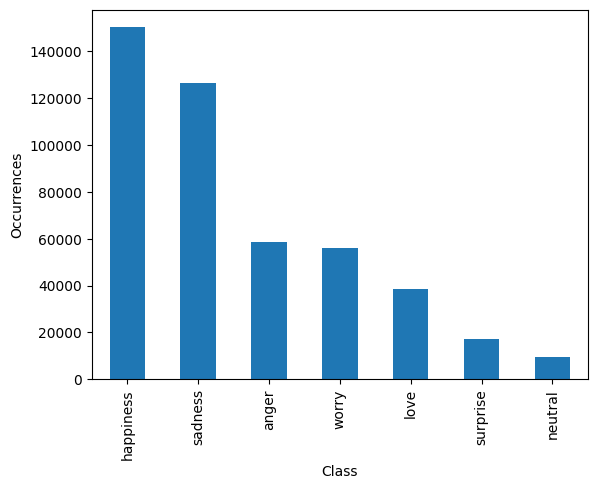
\includegraphics[width=0.48\textwidth]{assets/class_distribution.png}
    \captionof{figure}{Class distribution of the full dataset}
    \label{fig:class_distribution}
\endgroup

As shown in figure \ref{fig:class_distribution},
the dataset is unbalanced. The most common
emotion is Happiness, and the least common
is Neutral. This is because the larger dataset
(Emotions) does not contain the Neutral class.

\begingroup
    \centering
    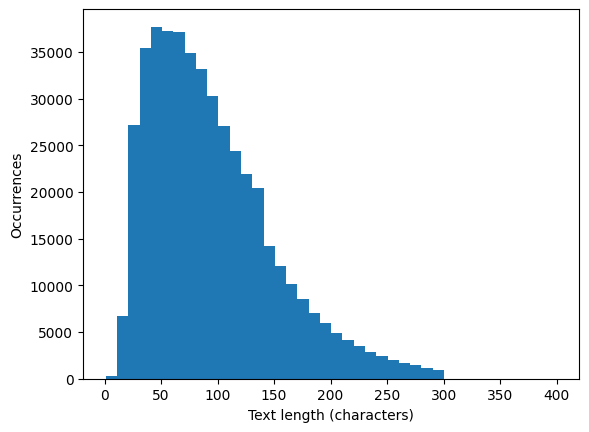
\includegraphics[width=0.48\textwidth]{assets/length_distribution.png}
    \captionof{figure}{Text length distribution of the full dataset}
    \label{fig:length_distribution}
\endgroup

The dataset was split into a training set
and a test set with a 80\% - 20\% ratio.

\subsection{Vectorization}
